\documentclass[]{article}

%opening
\title{{\bf Practical 1}: Predicting the Efficiency of Organic Photovoltaics}
\author{Neil Chainani
		Avery Faller}

\usepackage[OT1]{fontenc}
\usepackage[colorlinks,citecolor=blue,urlcolor=blue]{hyperref}
\usepackage[pdftex]{graphicx}
\usepackage{subfig}
\usepackage{fullpage}
\usepackage{palatino}
\usepackage{mathpazo}
\usepackage{amsmath}
\usepackage{amssymb}
\usepackage{color}
\usepackage{todonotes}
\usepackage{listings}
\usepackage[utf8]{inputenc}
\usepackage[english]{babel}

\definecolor{dkgreen}{rgb}{0,0.6,0}
\definecolor{gray}{rgb}{0.5,0.5,0.5}
\definecolor{mauve}{rgb}{0.58,0,0.82}

\lstset{frame=tb,
  language=Python,
  aboveskip=3mm,
  belowskip=3mm,
  showstringspaces=false,
  columns=flexible,
  basicstyle={\small\ttfamily},
  numbers=none,
  numberstyle=\tiny\color{gray},
  keywordstyle=\color{blue},
  commentstyle=\color{dkgreen},
  stringstyle=\color{mauve},
  breaklines=true,
  breakatwhitespace=true,
  tabsize=3
}

\renewcommand{\baselinestretch}{1.25	}




\begin{document}
	
\maketitle

\section{Technical Approach}
\subsection*{How did you tackle the problem?}
\begin{figure}[h]
	\centering
	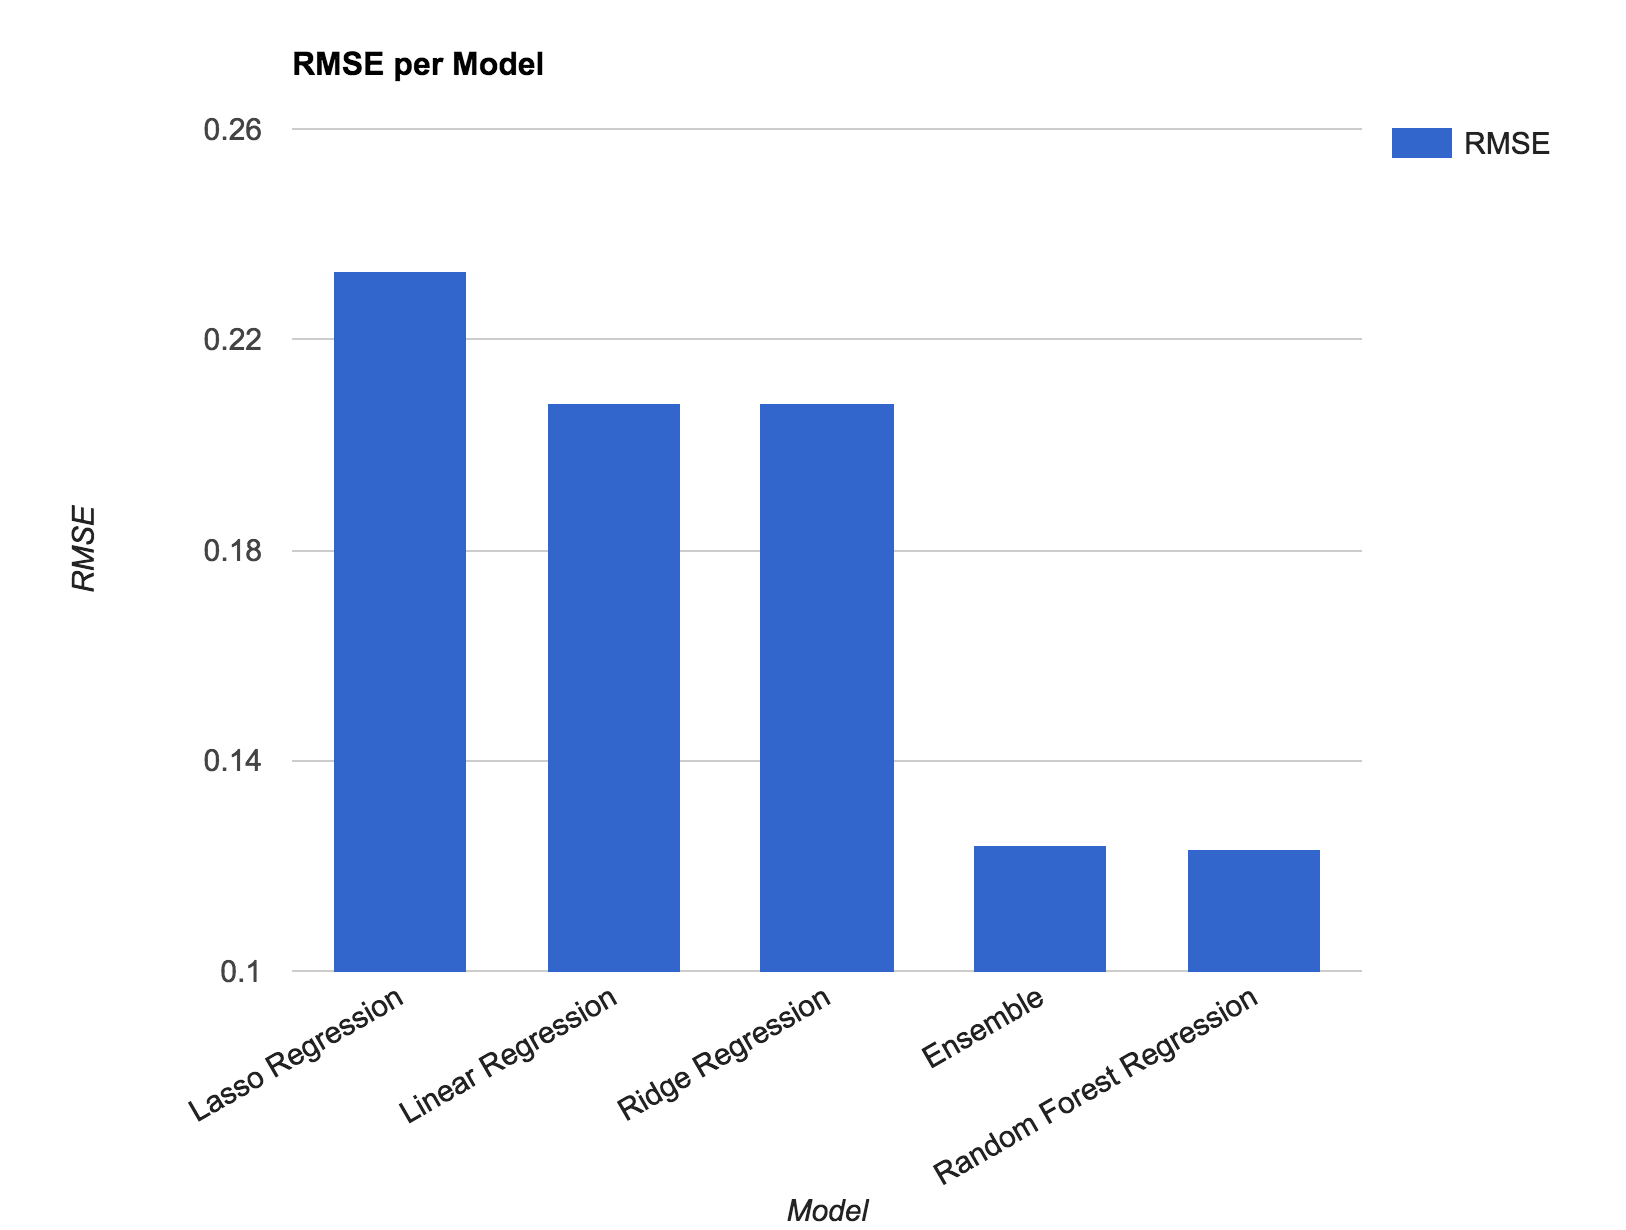
\includegraphics[width=0.7\textwidth]{ModelComparison}
	\caption{Comparison of unoptimized models}
\end{figure}

\begin{flushleft}
	We began with the supplied Sample IPython notebook, which applied basic linear regression and random forests on the 256 provided binary features. The first step in our approach was to determine the most effective machine learning model. We compared the root mean squared error (RMSE) for a number of unoptimized models, including Linear Regression, Lasso Regression, Ridge Regression, Random Forest Regression and an ensemble of the four, and determined that the Random Forest Regressor had the lowest RMSE. We also tried K-nearest neighbors, and Polynomial Interpolation, but Random Forest Regression was better and faster than both of them.
	\newline\newline
	Once we had established that Random Forest Regressors were the model to go with, we began the process of engineering the most effective features while simultaneously tuning our Random Forest Regressor to produce the best predictions.  We had a hunch that some of the given binary features were not useful, so we summed up each of the columns. We saw immediately that out of the 256 features, 244 of them had a value of 0 for every molecule, so we dropped these columns for the sake of efficiency.
	\newline\newline
	It was clear that the remaining provided binary features were hardly sufficient, so we decided to delve into the SMILES feature. This complex string held a wealth of information regarding the chemical properties of the molecule, however, neither of us have much domain knowledge in chemistry, so for our feature extraction, we mainly treated the SMILES as a text analysis problem.
	\newline\newline
	We first applied a basic set of features on the counts of the characters within the strings. We discovered that there were only 21 distinct case-sensitive characters present in the string, and added an indicator variable for each of these as a feature. 
	\newline\newline
	\begin{figure}[h]
		\centering
		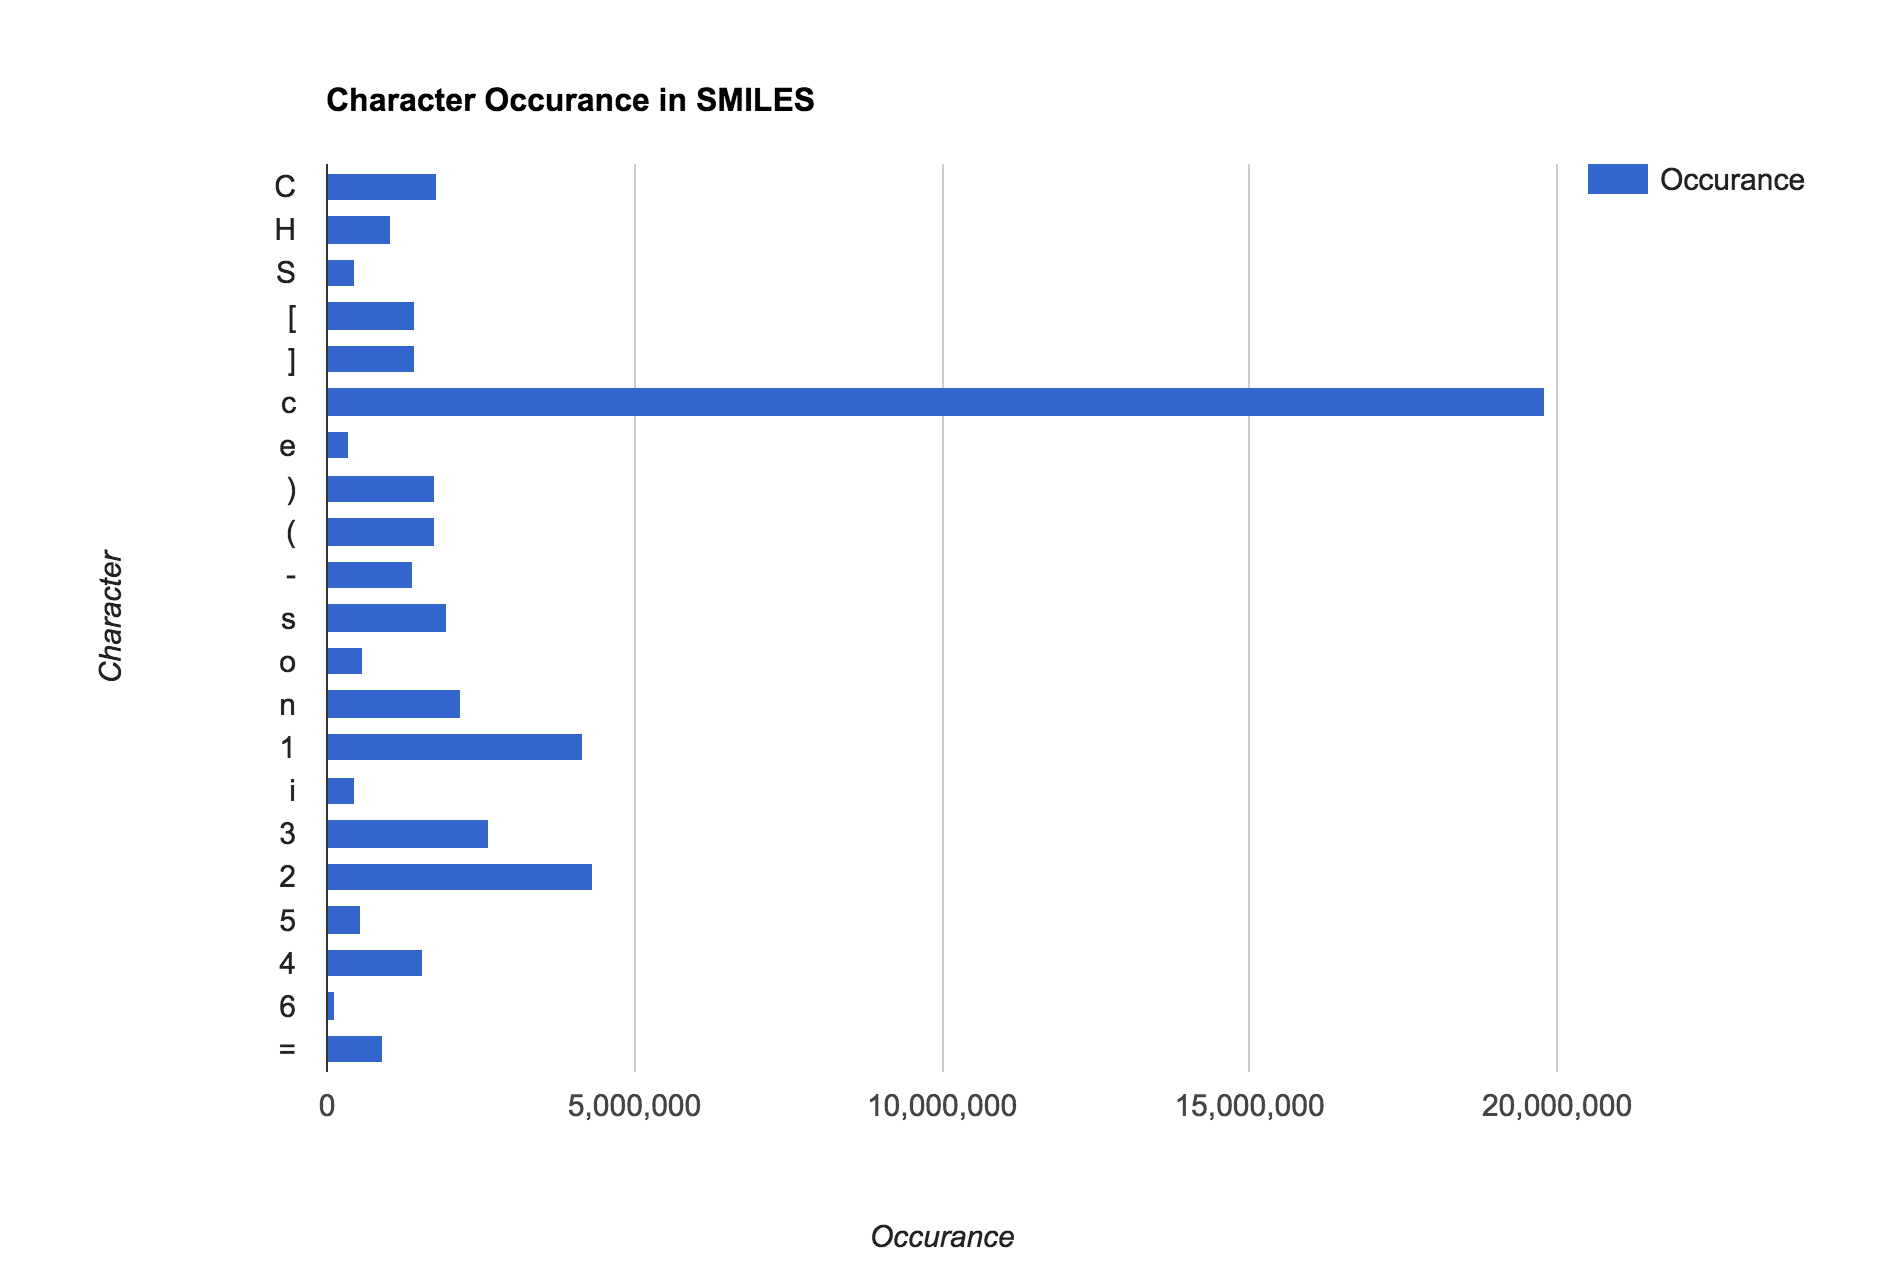
\includegraphics[width=0.8\textwidth]{CharacterOccurance}
		\caption{Occurrence counts of all 21 characters within the full training set}
	\end{figure}
	\newline\newline
	We then pursued more deliberate feature engineering using our limited knowledge of chemistry. We extracted features, such as the length of the SMILES string, the percentage of the SMILES string that was uppercase and lowercase (which indicates it is aromatic). We picked out specific molecules, such as ‘o1cccc1’ and ‘n1ccccc1’, and created indicator features for them.  Finally, we looked at whether the SMILES string began or ended with certain molecules. 
	\newline\newline
	The model continued to improve, but we were certain there was more manipulation to be done. Developing features by hand was time consuming, so we auto-generated features for the top N bi-grams (pairs of consecutive characters), and tuned the number N high enough until we saw diminishing returns given time constraints. Because of how much success this reaped, we repeated this process for 3-grams, 4-grams and 5-grams, and were able to bring our RMSE down significantly with each additional set of features.  However, as our RMSE improved, it became increasingly difficult to lower, and the runtime of our Random Forest Regressor increased dramatically.
	\newline\newline
\end{flushleft}
\section{Results}
\subsection*{How well did your set of predictions do?}
\begin{flushleft}
	\begin{figure}[h]
		\centering
		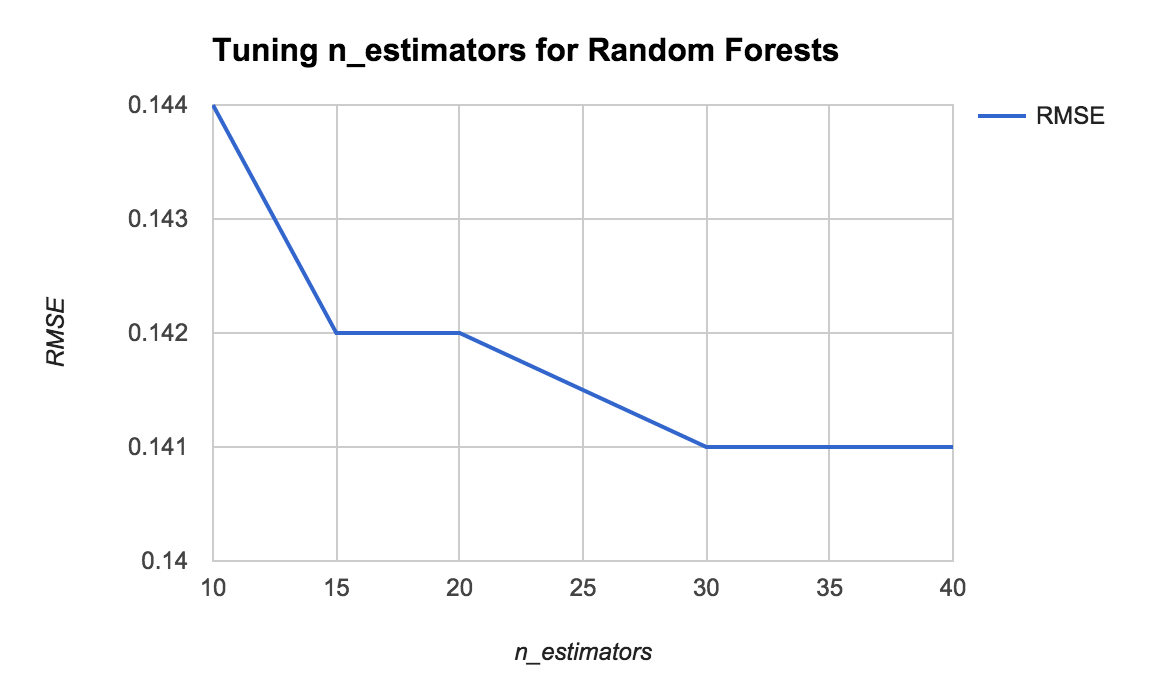
\includegraphics[width=0.8\textwidth]{n_estimators}
		\caption{Tuning number of trees for Random Forests.  We stopped at 40 because the improvements in RMSE were minimal compared with the extended time it took to fit the data with large numbers of trees.}
	\end{figure}
	We started from the Random Forest baseline given in the sample code.  This code generates predictions with a RMSE of .272.  Our biggest drop in RMSE was our first one.  By simply adding an indicator column for each symbol in the SMILES dictionary and iterating over hyperparameters for the Random Forest Regressor, we dropped our RMSE down to .141.
	\newline\newline
	After performing feature engineering to build up 50 custom features and tuning again, this time on the min\_samples\_split parameter, our RMSE dropped again to .1260. After this drop, it became much harder to improve. 
	\newline\newline
	\begin{figure}[h]
		\centering
		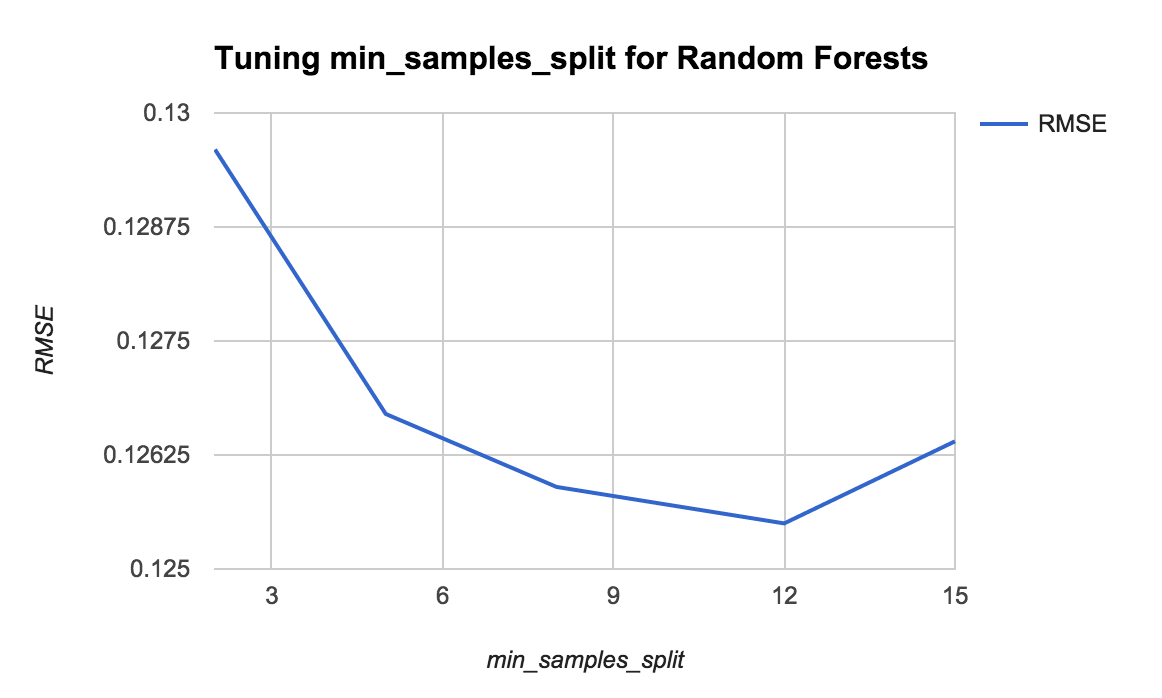
\includegraphics[width=0.8\textwidth]{min_samples_split}
		\caption{Tuning min samples split for Random Forests}
	\end{figure}
	\newline\newline
	Adding Bigrams and tuning how many we used brought us further down to .1011.  Continuing in this vein, we added Trigrams, which dropped us further down to .0864.  Quadgrams brought the RMSE to .0809 and Quintgrams further lowered the RMSE to .0777.
	\newline\newline
	All of this is to say that adding additional features continued to lower our RMSE, however these improvements came at the cost of potentially overfitting on the training set and significantly increasing our running time.  By the end, fitting the Random Forest took on the order of two hours when all of our features were turned on.
\end{flushleft}
\section{Discussion}
\subsection*{What was your thought process for your approach?}
\begin{flushleft}
	Our work had two major parts to it: selecting the best model, and engineering the best set of features.  Selecting the best model was mainly about testing, but those tests agreed with our thoughts:  Random Forests work best with lots of data, and we had no shortage of data in this Practical.  
	\newline\newline
	Random Forests also have the advantage of being less prone to overfitting.  So, with that fact in mind, we set about building lots of features to fit our model with.  We built around 50 features by hand that looked for specific molecules or other special features of the SMILES strings.  However, this was taking a long time to create features and test them, so we set about finding a way to automate feature creation.  
	\newline\newline
	We choose to do this by building N-grams, starting with monograms, and working our way up to quintgrams.  By simply piling lots of features into our dataframe, we were able to compensate for our limited understanding of chemistry by providing the regressor with a large quantity of features to fit on.  In the end we had over 600 features.  Although undoubtedly some of these features were quite bad, or even detrimental to the model, by providing enough of them with a sufficient amount of data (and in this practical we had no shortage of data), Random Forest Regression was able to discover which were the most significant and accurate predictors of the gap metric and exploit them.
	\newline\newline
	\begin{figure}[h]
		\centering
		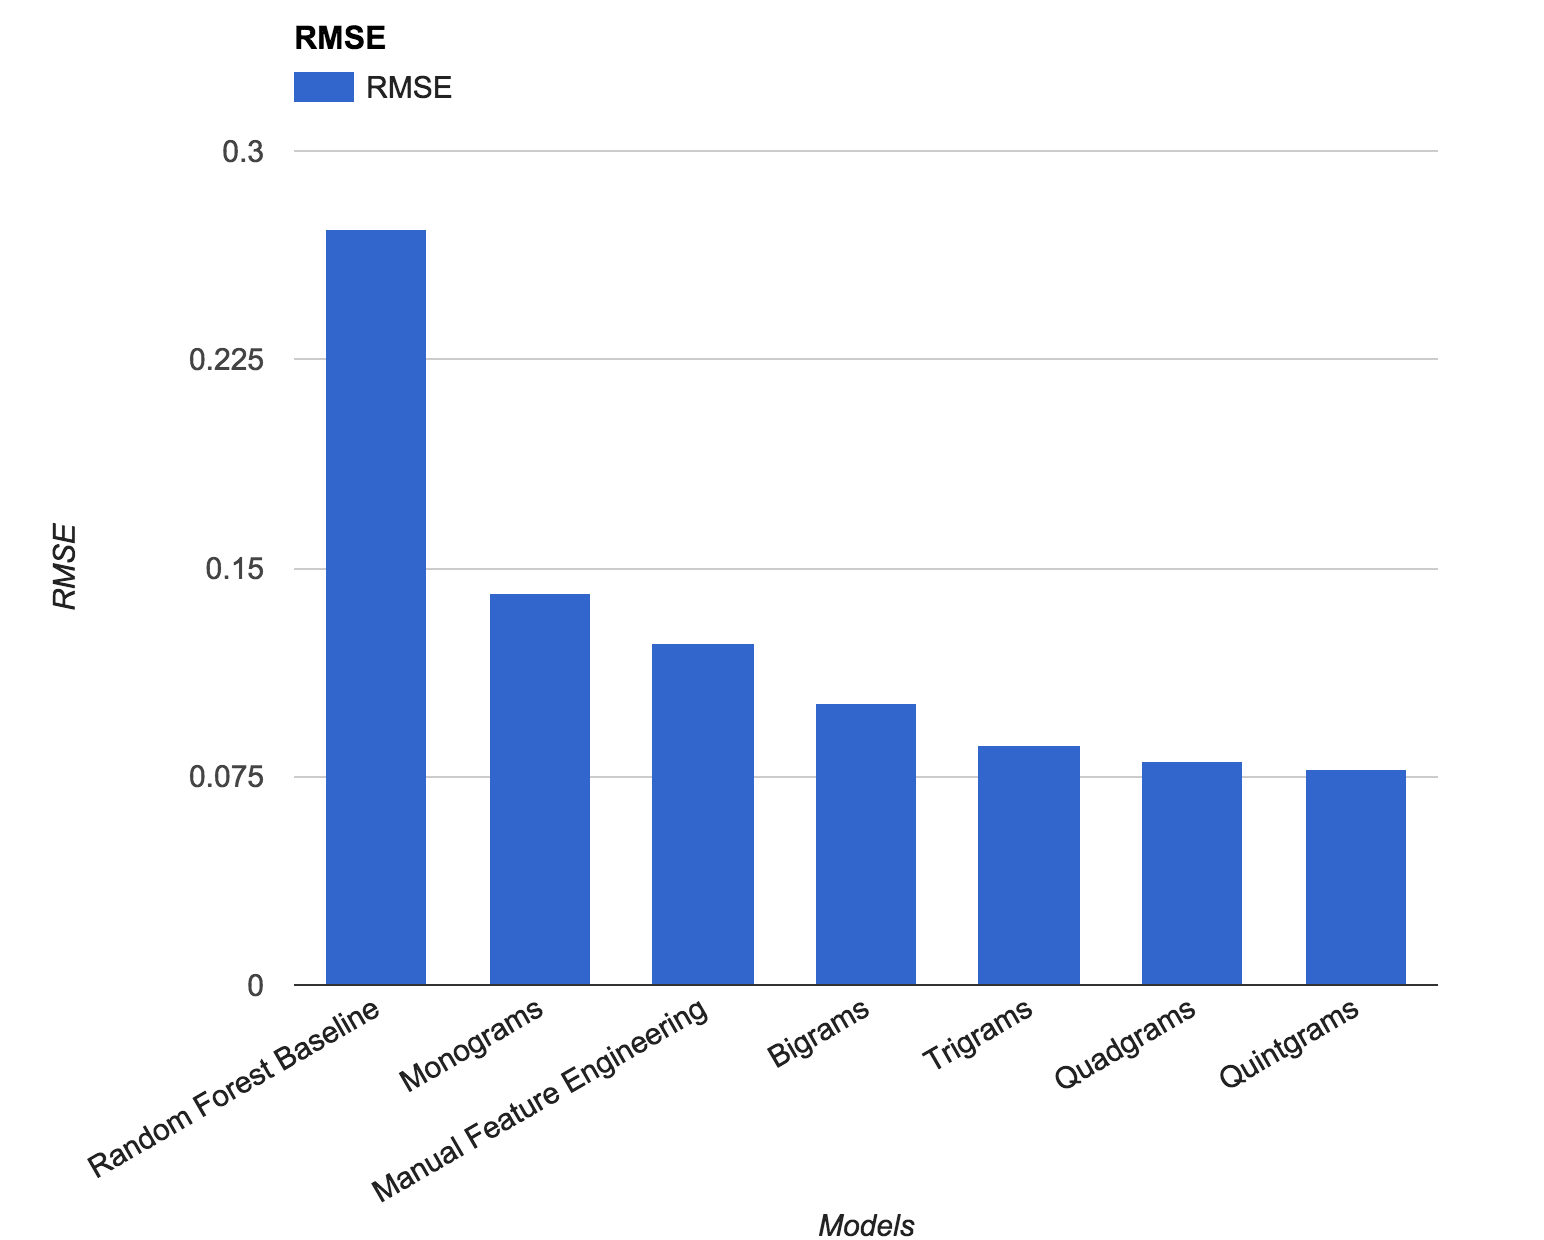
\includegraphics[width=0.8\textwidth]{RMSEperModel}
		\caption{Seeing the RMSE fall as we add complexity to the model.  However, gains become smaller and harder to achieve and our approach begins to level off towards the end.}
	\end{figure}
\end{flushleft}	
\newpage
\section{Code}
\subsection*{The Python code below can also be viewed on GitHub in iPython Notebook form at: https://github.com/averyfaller/CS181Practical/tree/master/1}
\begin{flushleft}
\begin{lstlisting}
# Imports
import pandas as pd
import numpy as np
import matplotlib.pyplot as plt
from sklearn.linear_model import LinearRegression
from sklearn.ensemble import RandomForestRegressor
from sklearn.cross_validation import train_test_split
from collections import Counter

# Make the DataFrame
df_train = pd.read_csv("train.csv")
df_test = pd.read_csv("test.csv")
# Store gap values
Y_train = df_train.gap.values
# Row where testing examples start
test_idx = df_train.shape[0]
# Delete 'Id' column
df_test = df_test.drop(['Id'], axis=1)
# Delete 'gap' column
df_train = df_train.drop(['gap'], axis=1)
# DataFrame with all train and test examples so we can more easily apply feature engineering on
df_all = pd.concat((df_train, df_test), axis=0)
df_all.head()

# A method to make features on a supplied DataFrame
def makeFeatures(df):
    
    ##########################
    ### DROP EMPTY COLUMNS ###
    ##########################
    # Remove 0 columns (columns with no data)
    zero_cols = []
    for i in range(1,257):
        if df['feat_%03d' % i].sum() == 0:
            zero_cols.append('feat_%03d' % i)
    df = df.drop(zero_cols, axis=1)
    
    ##############################
    ### SMILE CHARACTER COUNTS ###
    ##############################
    smiles = df.smiles
    smileydict = smiles.map(lambda x: dict(Counter(x)))
    smile_alphabet=list(set(''.join(smiles.iloc[0:50])))
    for smile in smile_alphabet:
        smilechar = smile
        if smile == '=':
            smilechar = 'equal'
        df['smile_'+smilechar] = smileydict.map(lambda x: x[smile] if smile in x.keys() else 0)
    
    ###########################
    ### FEATURE ENGINEERING ###
    ###########################
    # Add length of smile
    df['smile_length'] = df.smiles.map(lambda x: len(x))

    # Add number of C's divided by length
    df['smile_percentc'] = (df.smile_c / df.smile_length)
    df['smile_percentC'] = (df.smile_C / df.smile_length)

    # Count specific molecules
    # [nH]
    df['smile_nh'] = df.smiles.map(lambda x: '[nH]' in x)
    df['smile_nh1'] = df.smiles.map(lambda x: '[nH]1' in x)
    df['smile_si'] = df.smiles.map(lambda x: 'Si' in x)
    df['smile_sih2'] = df.smiles.map(lambda x: '[SiH2]' in x)
    df['smile_se'] = df.smiles.map(lambda x: '[se]' in x)
    df['smile_CdoubleC'] = df.smiles.map(lambda x: 'C=C' in x)
    df['smile_doubleC'] = df.smiles.map(lambda x: 'CC' in x)
    df['smile_doublec'] = df.smiles.map(lambda x: 'cc' in x)
    df['smile_triplec'] = df.smiles.map(lambda x: 'ccc' in x)
    df['smile_quadc'] = df.smiles.map(lambda x: 'cccc' in x)
    df['smile_quintc'] = df.smiles.map(lambda x: 'ccccc' in x)
    df['smile_C1equalCc2'] = df.smiles.map(lambda x: 'C1=Cc2' in x)
    df['smile_C1'] = df.smiles.map(lambda x: 'C1' in x)
    df['smile_c1'] = df.smiles.map(lambda x: 'c1' in x)
    df['smile_equalCCCequal'] = df.smiles.map(lambda x: '=CCC=' in x)
    df['smile_equalCCequal'] = df.smiles.map(lambda x: '=CC=' in x)
    df['smile_equalCequal'] = df.smiles.map(lambda x: '=C=' in x)
    df['smile_C1equalCCequalC'] = df.smiles.map(lambda x: 'C1=CC=C' in x)
    df['smile_c1cccs1'] = df.smiles.map(lambda x: 'c1ccc(s1)' in x)

    # Important molecules
    df['smile_c1ccccc1'] = df.smiles.map(lambda x: 'c1ccccc1' in x)
    df['smile_n1ccccc1'] = df.smiles.map(lambda x: 'n1ccccc1' in x)
    df['smile_o1cccc1'] = df.smiles.map(lambda x: 'o1cccc1' in x)
    df['smile_c1ccccc1-c2ccccc2'] = df.smiles.map(lambda x: 'c1ccccc1-c2ccccc2' in x)
    df['smile_n1c[nH]cc1'] = df.smiles.map(lambda x: 'n1c[nH]cc1' in x)
    
    # Parentheses molecules
    df['smile_parenC1'] = df.smiles.map(lambda x: '(C1)' in x)
    df['smile_parenc1'] = df.smiles.map(lambda x: '(c1)' in x)
    df['smile_parencc1'] = df.smiles.map(lambda x: '(cc1)' in x)
    df['smile_pareno1'] = df.smiles.map(lambda x: '(o1)' in x)
    df['smile_parens1'] = df.smiles.map(lambda x: '(s1)' in x)
    df['smile_parenccc4mol'] = df.smiles.map(lambda x: '(ccc4=C[SiH2]C=c34)' in x)
    df['smile_parenccinnermol'] = df.smiles.map(lambda x: '(cc(-c3ccco3)c3=CCC=c13)' in x)
    df['smile_parennegc3cco3'] = df.smiles.map(lambda x: '(-c3ccco3)' in x)
    df['smile_parenncc3c12'] = df.smiles.map(lambda x: '(ncc3c12)' in x)
    df['smile_parenccc34'] = df.smiles.map(lambda x: '(ccc34)' in x)
    df['smile_parencc4ccc3c2cn1'] = df.smiles.map(lambda x: '(cc4ccc3c2cn1)' in x)

    # Special
    df['smile_percent_aromatic'] = (df.smile_c + df.smile_o + df.smile_n + df.smile_s / df.smile_length)

    # Start
    df['smile_start_C1'] = df.smiles.map(lambda x: x.startswith('C1'))
    df['smile_start_C1equal'] = df.smiles.map(lambda x: x.startswith('C1='))
    df['smile_start_c1'] = df.smiles.map(lambda x: x.startswith('c1'))
    df['smile_start_cc1'] = df.smiles.map(lambda x: x.startswith('cc1'))
    df['smile_start_c1sc'] = df.smiles.map(lambda x: x.startswith('c1sc'))
    df['smile_start_c1ccc'] = df.smiles.map(lambda x: x.startswith('c1ccc'))
    df['smile_start_nH'] = df.smiles.map(lambda x: x.startswith('[nH]'))
    df['smile_start_C1equalCCequalC'] = df.smiles.map(lambda x: x.startswith('C1=CC=C'))

    # End
    df['smile_end_c1ccc'] = df.smiles.map(lambda x: x.endswith('c1ccc'))
    df['smile_end_o1'] = df.smiles.map(lambda x: x.endswith('o1'))
    df['smile_end_ccsc12'] = df.smiles.map(lambda x: x.endswith('ccsc12'))
    
    joint = ''.join(smiles.iloc[:3000])
    
    ###############
    ### BIGRAMS ###
    ###############
    top_50_bigrams = Counter(zip(joint,joint[1:])).most_common(200)
    for bigram,count in top_50_bigrams:
        b = bigram[0]+bigram[1]+""
        df[b+"_bigram"] = smiles.map(lambda x: 1 if b in x else 0)
        
    ################
    ### TRIGRAMS ###
    ################
    top_trigrams = Counter(zip(joint, joint[1:], joint[2:])).most_common(200)
    for trigram, count in top_trigrams:
        t = trigram[0]+trigram[1]+trigram[2]+""
        df[t+"_trigram"] = smiles.map(lambda x: 1 if t in x else 0)
        
    ################
    ### QUADGRAMS ###
    ################
    top_quadgrams = Counter(zip(joint, joint[1:], joint[2:], joint[3:])).most_common(100)
    for quadgram, count in top_quadgrams:
        q = quadgram[0]+quadgram[1]+quadgram[2]+quadgram[3]+""
        df[q+"_quadgram"] = smiles.map(lambda x: 1 if q in x else 0)
        
    ################
    ### QUINTS ###
    ################
    top_quintgrams = Counter(zip(joint, joint[1:], joint[2:], joint[3:], joint[4:])).most_common(100)
    for quintgram, count in top_quintgrams:
        q = quintgram[0]+quintgram[1]+quintgram[2]+quintgram[3]+quintgram[4]+""
        df[q+"_quintgram"] = smiles.map(lambda x: 1 if q in x else 0)
    
    ################################
    ### DROP UNNECESSARY COLUMNS ###
    ################################   
    df = df.drop('smile_length', axis=1)
    
    return df

# Make the features
print "Making Features"
df_all = makeFeatures(df_all)
df_all.shape

# Split the train and test sets
df_all = df_all.drop(['smiles'], axis=1)
vals = df_all.values
X_train = vals[:test_idx]
X_test = vals[test_idx:]
print "Train features:", X_train.shape
print "Train gap:", Y_train.shape
print "Test features:", X_test.shape

# Create temporary train, validate and test sets from the X_train set
X_tmp_trainvalidate, X_tmp_test, Y_tmp_trainvalidate, Y_tmp_test = train_test_split(X_train, Y_train, test_size=0.20, random_state=37)
X_tmp_train, X_tmp_validate, Y_tmp_train, Y_tmp_validate = train_test_split(X_tmp_trainvalidate, Y_tmp_trainvalidate, test_size=0.20, random_state=42)

# Validate and tune the Random Forest Regressor
bestRFValidateRMSE = 1.0
bestRFN = 10
bestRFS = 2

for n in [40, 50]:
    for s in [12]:
        RF = RandomForestRegressor(n_estimators=n, min_samples_split=s)
        RF.fit(X_tmp_train, Y_tmp_train)
        rmse = np.sqrt(np.mean((RF.predict(X_tmp_validate) - Y_tmp_validate) ** 2))
        print("Validation RMSE for n = %d, min_samples_split = %d: %.4f" % (n, s, rmse))
        if (rmse < bestRFValidateRMSE):
            bestRFValidateRMSE = rmse
            bestRFN = n
            bestRFS = s

print "The best N for RF was: %d, with min_samples_split: %d, with RMSE: %.4f" % (bestRFN, bestRFS, bestRFValidateRMSE)

# Test the final settings for the Random Forest Regressor
print "BEST RF N: %d" % bestRFN
RF = RandomForestRegressor(n_estimators=bestRFNn, min_samples_split=bestRFS)
RF.fit(X_tmp_train, Y_tmp_train)
print("Test RMSE: %.4f" % np.sqrt(np.mean((RF.predict(X_tmp_test) - Y_tmp_test) ** 2)))

# Fit the Random Forest on the full X_train set
RF = RandomForestRegressor(n_estimators=bestRFN, min_samples_split=bestRFS)
RF.fit(X_train, Y_train)
RF_pred = RF.predict(X_test)

def write_to_file(filename, predictions):
    with open(filename, "w") as f:
        f.write("Id,Prediction\n")
        for i,p in enumerate(predictions):
            f.write(str(i+1) + "," + str(p) + "\n")
            
write_to_file("prediction.csv", RF_pred)
\end{lstlisting}


\end{flushleft}	

\end{document}
